
\documentclass [a4paper] {article}
\usepackage[utf8]{inputenc}
\title{Ciencia de datos, práctica 1}
\author{Juan Casado Ballesteros}
\usepackage{Sweave}
\begin{document}
\maketitle

\begin{abstract}
En esta práctica vamos a realizar tres análisis estadísticos, 
en los dos primeros utilizaremos las funciones propias de R sobre los datos proporcionados por el profesor en los formatos .txt para el primero y .sav para el segundo.
En el tercer análisis hemos programado nosotros mismos nuestras propias funciones. 
Como datos hemos elegido un .csv que contiene información sobre el alquiler en la Ciudad de Nueva York.
Intentaremos para este tercer análisis realizar un estudio crítico que nos permita llegar a conocer los datos con los que estamos trabajando.
\end{abstract}

\tableofcontents
\newpage

%-----------------------------------------------------------------------------------------------------------------------------------------------------------------------
\section{Primer análisis satelites menores de urano.txt}
%-----------------------------------------------------------------------------------------------------------------------------------------------------------------------

Comenzamos leyendo los datos del archivo .txt ya que dicho archivo lo hemos escrito con la sintaxis que textbf{read.table} espera 
por lo que no tendremos que utilizar ningún parámetro adicional para configurar la lectura de los datos.
\begin{Schunk}
\begin{Sinput}
> source("init.R")
> satelites <- read.table("./satelites.txt")
\end{Sinput}
\end{Schunk}

Primero calcularemos la frecuencia absoluta de los datos, que es el número de apariciones de cada uno de ellos.

\begin{Schunk}
\begin{Sinput}
> frecuencia_absoluta<-table(satelites$radio)
\end{Sinput}
\end{Schunk}
\begin{center}
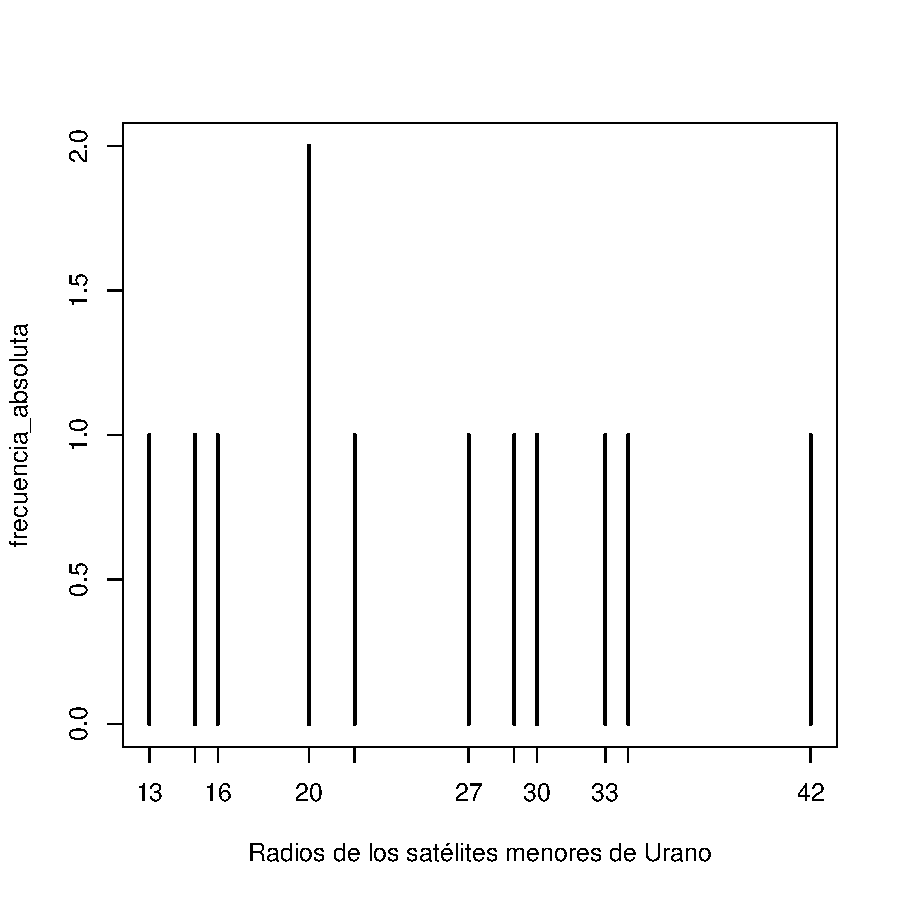
\includegraphics{entrega-frecuencia_absoluta_satelites_plot}
\end{center}

Ahora calcularemos la frecuencia absoluta acumulada.

\begin{Schunk}
\begin{Sinput}
> frecuencia_absoluta_acumulada<-cumsum(frecuencia_absoluta)
\end{Sinput}
\end{Schunk}
\begin{center}
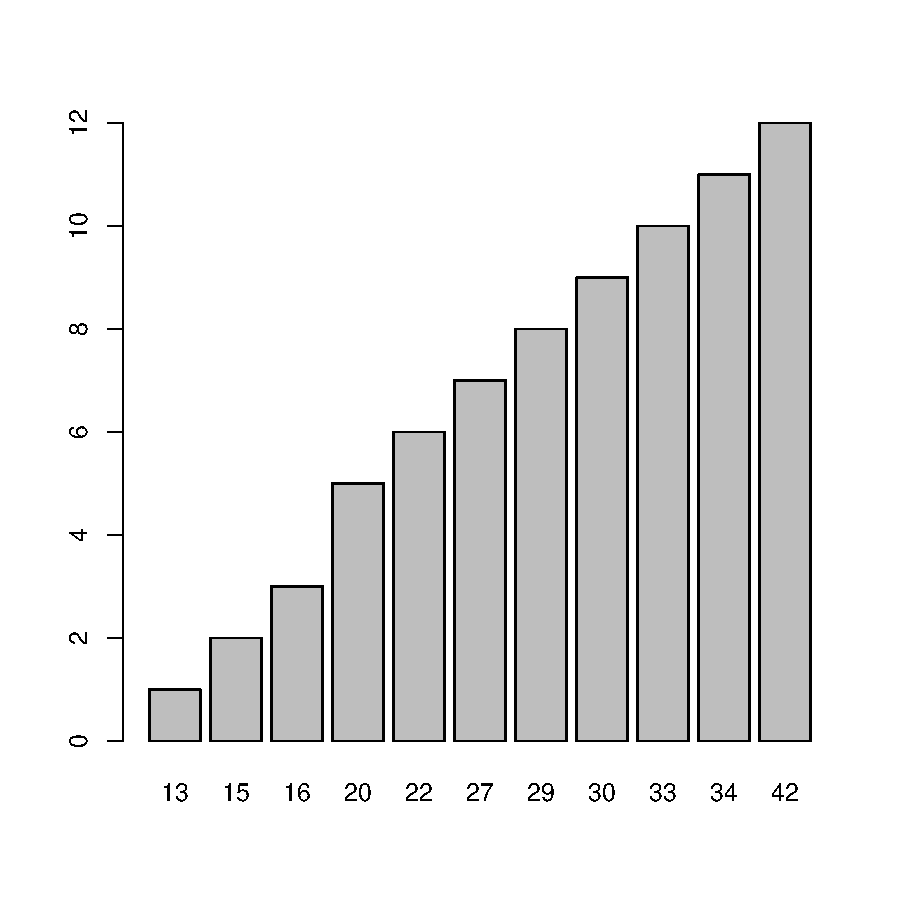
\includegraphics{entrega-frecuencia_absoluta_acumulada_satelites_plot}
\end{center}

Ahora calcularemos la frecuencia relativa.

\begin{Schunk}
\begin{Sinput}
> frecuencia_relativa <- (function(data) table(data)/length(data))(satelites$radio)
> sum(frecuencia_relativa)
\end{Sinput}
\begin{Soutput}
[1] 1
\end{Soutput}
\end{Schunk}
\begin{center}
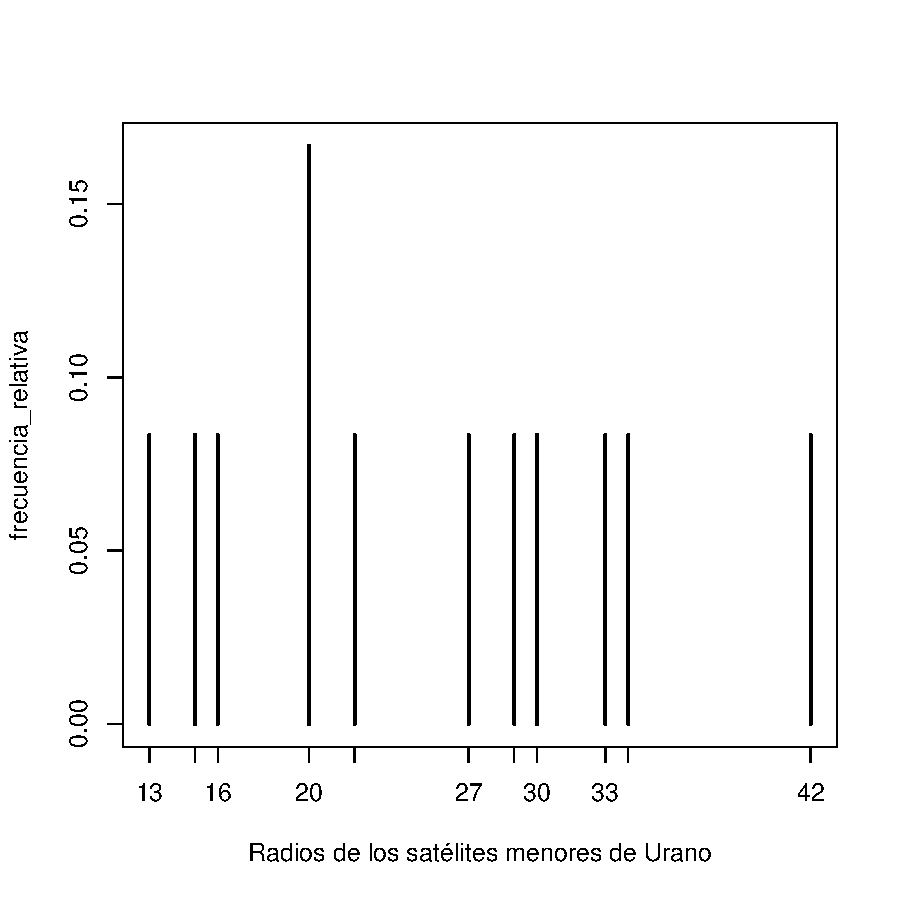
\includegraphics{entrega-frecuencia_relativa_satelites_plot}
\end{center}

Ahora calcularemos la frecuencia relativa acumulada.

\begin{Schunk}
\begin{Sinput}
> frecuencia_relativa_acumulada <- cumsum(frecuencia_relativa)
\end{Sinput}
\end{Schunk}
\begin{center}
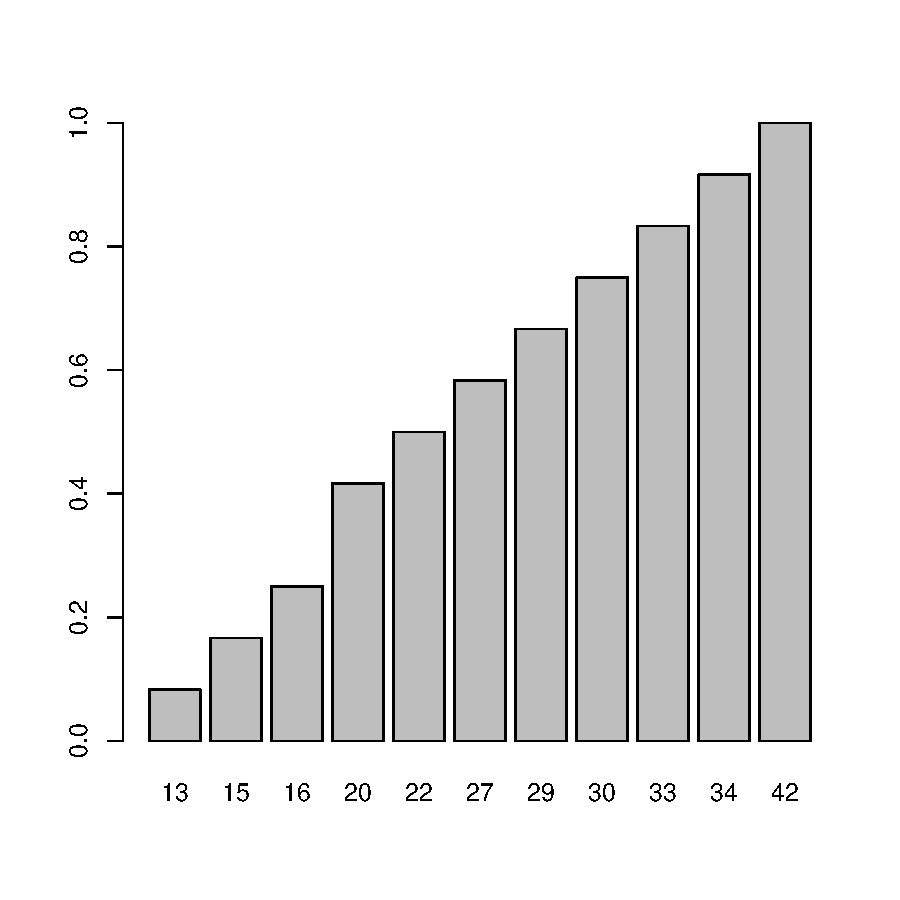
\includegraphics{entrega-frecuencia_relativa_acumulada_satelites_plot}
\end{center}

Calcularemos a continuación estadísticos cuya función es resumir los datos de los que disponemos.
Estos estadísticos son la media, la moda y la mediana.

\begin{Schunk}
\begin{Sinput}
> media <- mean(satelites$radio)
> v_mediana <- median(satelites$radio)
> v_moda <- moda(satelites$radio)
> desviacion_tipica <- sd(satelites$radio)
> v_varianza <- var(satelites$radio)
\end{Sinput}
\end{Schunk}
\begin{center}
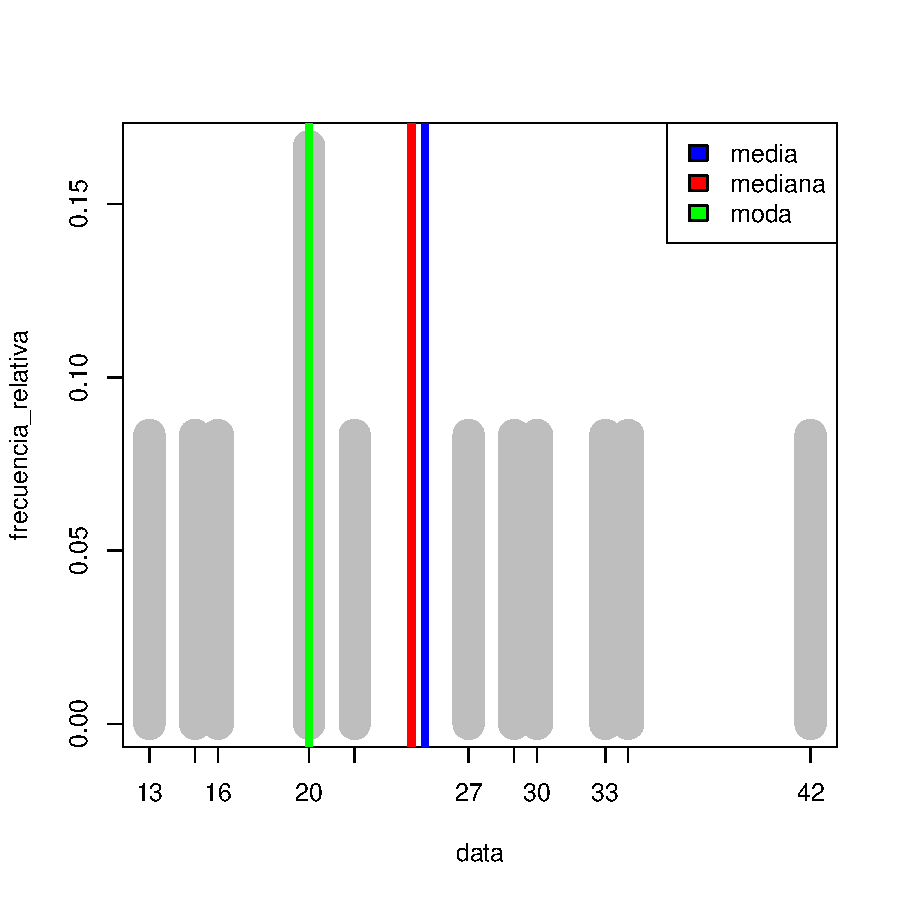
\includegraphics{entrega-estadisticos_satelites_plot}
\begin{Schunk}
\begin{Sinput}
> desviacion_tipica
\end{Sinput}
\begin{Soutput}
[1] 8.857029
\end{Soutput}
\begin{Sinput}
> v_varianza
\end{Sinput}
\begin{Soutput}
[1] 78.44697
\end{Soutput}
\end{Schunk}
\end{center}

Cuantiles y cuartiles ...
\begin{Schunk}
\begin{Sinput}
> v_cuartiles <- quantile(satelites$radio, prob=c(0, .25, .5, .75, 1))
> v_cuantil54 <- quantile(satelites$radio, prob=(.54))
\end{Sinput}
\end{Schunk}
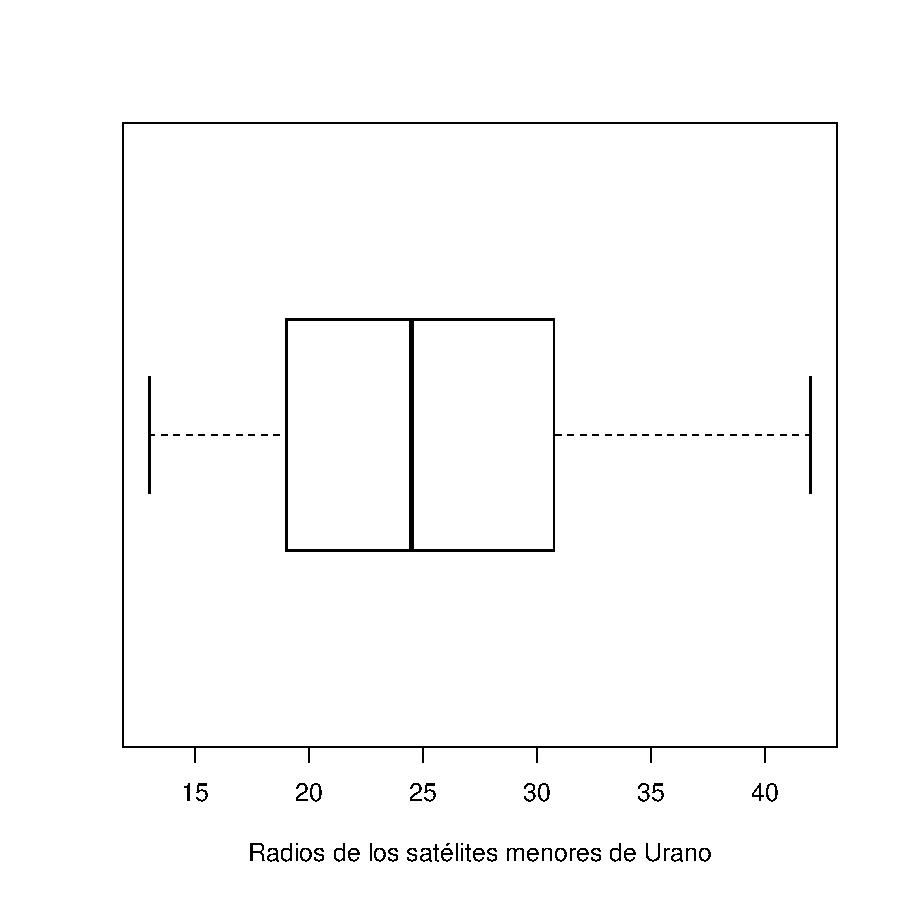
\includegraphics{entrega-cuartiles_satelites_plot}
\begin{Schunk}
\begin{Sinput}
> v_cuartiles
\end{Sinput}
\begin{Soutput}
   0%   25%   50%   75%  100% 
13.00 19.00 24.50 30.75 42.00 
\end{Soutput}
\begin{Sinput}
> v_cuantil54
\end{Sinput}
\begin{Soutput}
 54% 
26.7 
\end{Soutput}
\end{Schunk}

%-----------------------------------------------------------------------------------------------------------------------------------------------------------------------
\section{Segundo análisis cardata .sav}
%-----------------------------------------------------------------------------------------------------------------------------------------------------------------------

\begin{Schunk}
\begin{Sinput}
> source("init.R")
> cardata <- read.spss("./cardata.sav")$mpg
> cardata <- cardata[!is.na(cardata)]
\end{Sinput}
\end{Schunk}

\begin{Schunk}
\begin{Sinput}
> mean(cardata)
\end{Sinput}
\begin{Soutput}
[1] 28.79351
\end{Soutput}
\begin{Sinput}
> median(cardata)
\end{Sinput}
\begin{Soutput}
[1] 28.9
\end{Soutput}
\begin{Sinput}
> moda(cardata)
\end{Sinput}
\begin{Soutput}
[1] 36
\end{Soutput}
\begin{Sinput}
> sd(cardata)
\end{Sinput}
\begin{Soutput}
[1] 7.37721
\end{Soutput}
\begin{Sinput}
> var(cardata)
\end{Sinput}
\begin{Soutput}
[1] 54.42323
\end{Soutput}
\end{Schunk}
\begin{center}
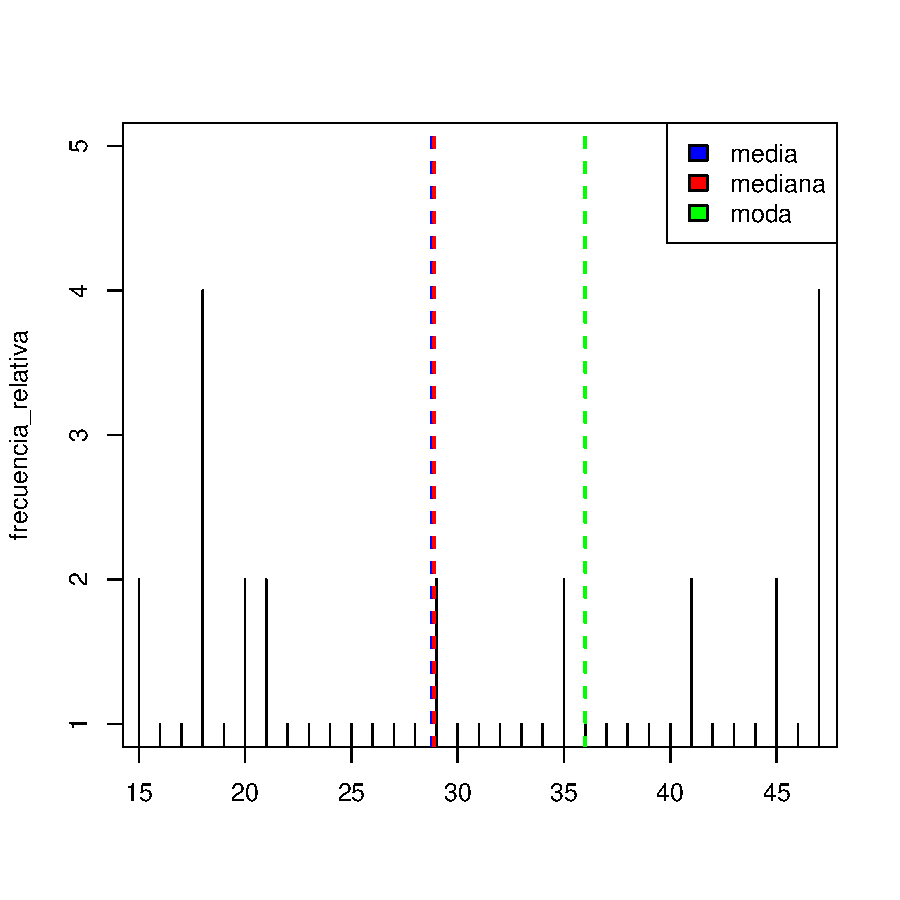
\includegraphics{entrega-018}
\end{center}
\begin{Schunk}
\begin{Sinput}
> v_cuartiles <- quantile(cardata, prob=c(0, .25, .5, .75, 1))
> v_cuartiles
\end{Sinput}
\begin{Soutput}
    0%    25%    50%    75%   100% 
15.500 22.550 28.900 34.275 46.600 
\end{Soutput}
\end{Schunk}
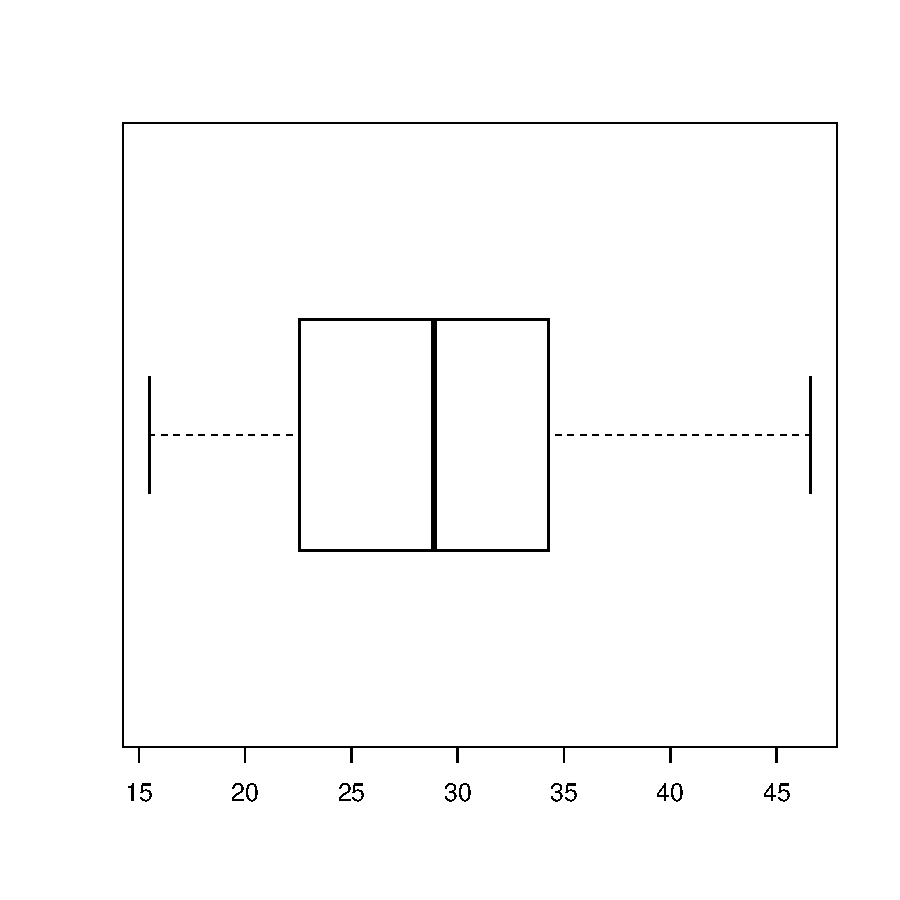
\includegraphics{entrega-020}


%-----------------------------------------------------------------------------------------------------------------------------------------------------------------------
\section{Tercer análisis del alquiler en Nueva York con AirBNB durante 2019 .csv}
%-----------------------------------------------------------------------------------------------------------------------------------------------------------------------

Haremos ahora un análisis de los datos del alquiler en la ciudad de Nueva York durante el año 2019 con la compañía AirBNB.
Los datos contienen las siguientes categorías:
\begin{Schunk}
\begin{Sinput}
> getInfo(data)
\end{Sinput}
\begin{Soutput}
                               unlist.res.
id                                 integer
name                                factor
host_id                            integer
host_name                           factor
neighbourhood_group                 factor
neighbourhood                       factor
latitude                           numeric
longitude                          numeric
room_type                           factor
price                              integer
minimum_nights                     integer
number_of_reviews                  integer
last_review                         factor
reviews_per_month                  numeric
calculated_host_listings_count     integer
availability_365                   integer
res_frame
 factor integer numeric 
      6       7       3 
\end{Soutput}
\end{Schunk}
Comenzaremos por analizar el precio de los alquileres.
Para ello calcularemos la frecuencia relativa de los precios.
\begin{Schunk}
\begin{Sinput}
> frecuencia_relativa<-frecuenciaRelativa(data$price)
\end{Sinput}
\end{Schunk}
\begin{center}
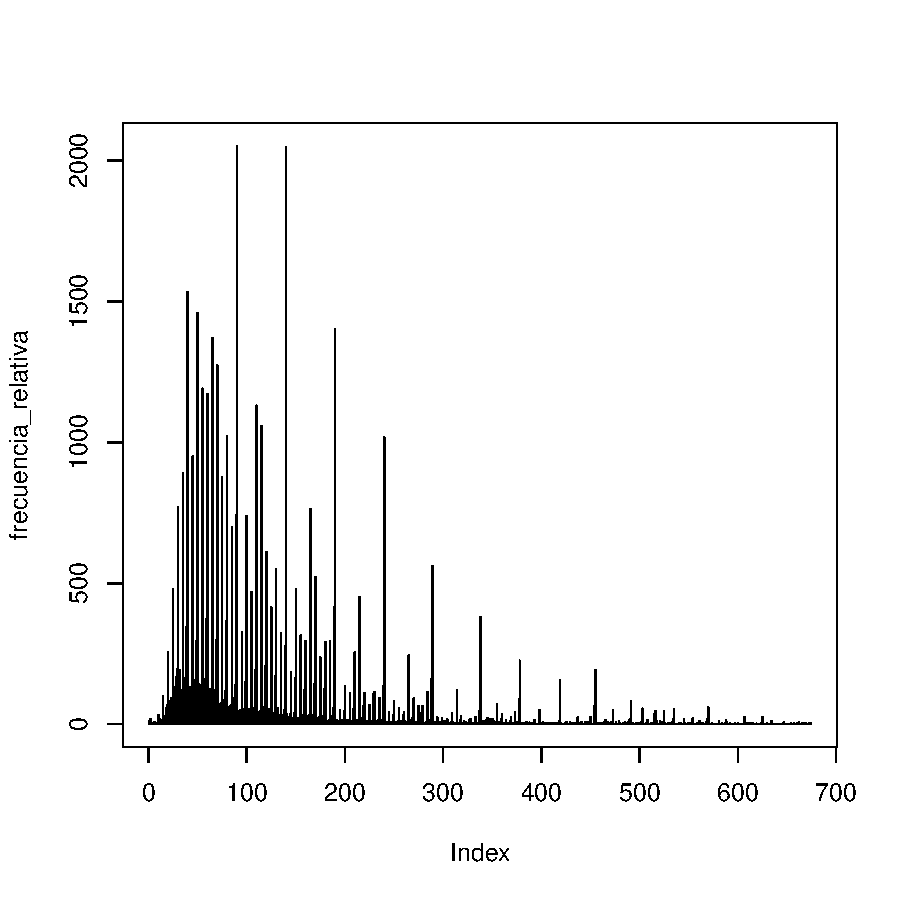
\includegraphics{entrega-frecuencia_relativa_BNB_plot}
\end{center}

Podemos observar que los precios están muy agrupados en la parte izquierda de la gráfica (precios bajos) con altos porcentajes de aparición,
no obstante aunque con una densidad mucho menor estos se alejan en gran medida llegando a alcanzar precios muy elevados pero con pocos porcentajes de aparición.

\begin{center}
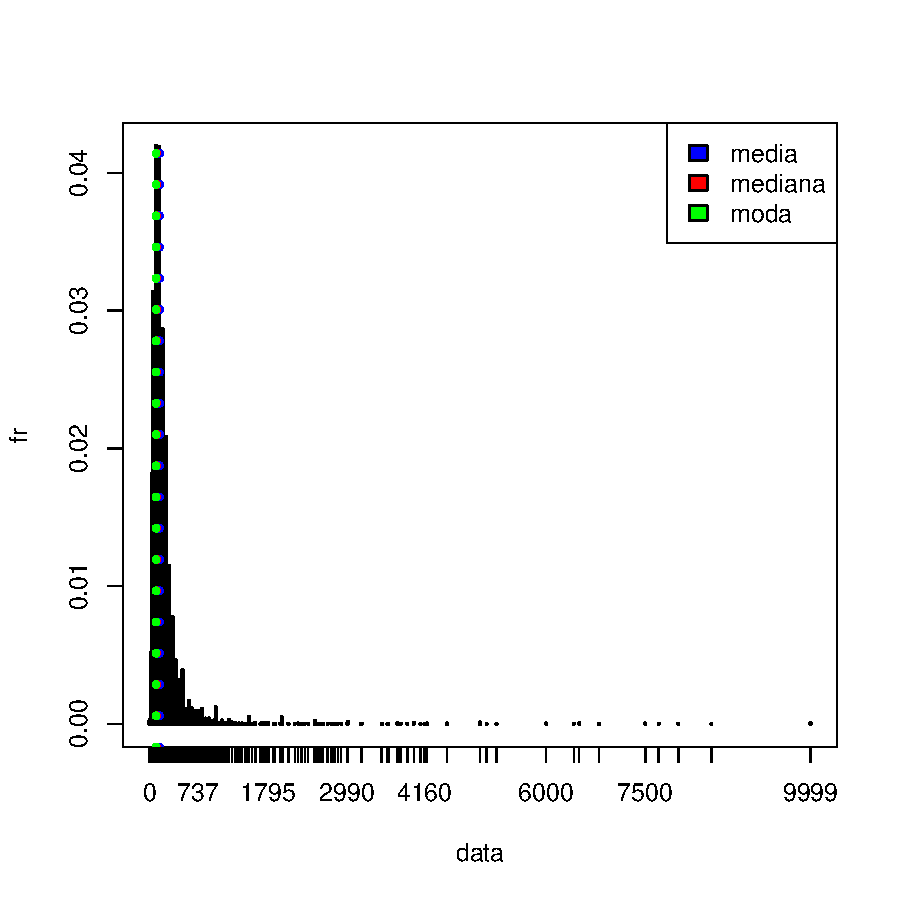
\includegraphics{entrega-estadisticos_BNB_plot}
\end{center}

\begin{Schunk}
\begin{Sinput}
> v_cuartiles <- cuartiles(data$price)
\end{Sinput}
\end{Schunk}
\begin{center}
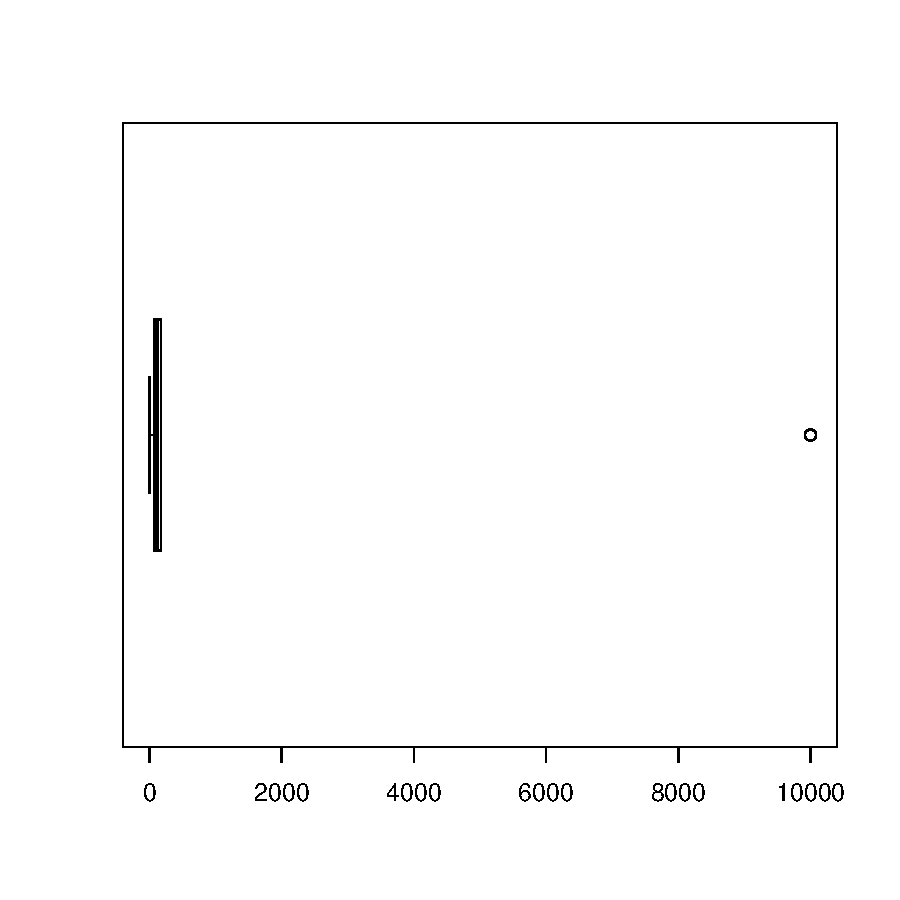
\includegraphics{entrega-cuartiles_BNB_plot}
\end{center}

Vemos que la media no es un valor representativo, su desviación típica es muy alta.
Podemos observar como la moda y la mediana en este caso parecen representar mejor a la mayoría de los datos.
Debido a esto decidimos que hacer el análisis de los precios para toda la ciudad no iba a aportarnos una visión representativa de los datos.
Decidimos ahora calcular el precio medio por cada barrio en vez de hacerlo sobre toda la ciudad a la vez.

\begin{Schunk}
\begin{Soutput}
        Group.1   x.media x.desviacion_tipica x.mediana    x.moda
1         Bronx  87.49679           106.66043  65.00000  60.00000
2      Brooklyn 124.38321           186.86889  90.00000 100.00000
3     Manhattan 196.87581           291.37646 150.00000 150.00000
4        Queens  99.51765           167.08741  75.00000  50.00000
5 Staten Island 114.81233           277.24801  75.00000  75.00000
\end{Soutput}
\end{Schunk}
Valores sobre el total de los datos sin haber separado por barrios
\begin{Schunk}
\begin{Soutput}
            media desviacion_tipica         v_mediana            v_moda 
         152.7207          240.1517          106.0000          100.0000 
\end{Soutput}
\end{Schunk}

Podemos ver que la varianza se ha reducido para más barrios de en los que ha aumentado.
En Bronx es en el barrio en el que tanto la varianza como la media es menor y 
Manhattan es en el que ambas son mayores.

Datos para Manhattan
\begin{center}
\begin{Schunk}
\begin{Sinput}
> manhattan_data = data$price[data$neighbourhood_group == "Manhattan"]
> plotFrecuencyData(manhattan_data)
\end{Sinput}
\end{Schunk}
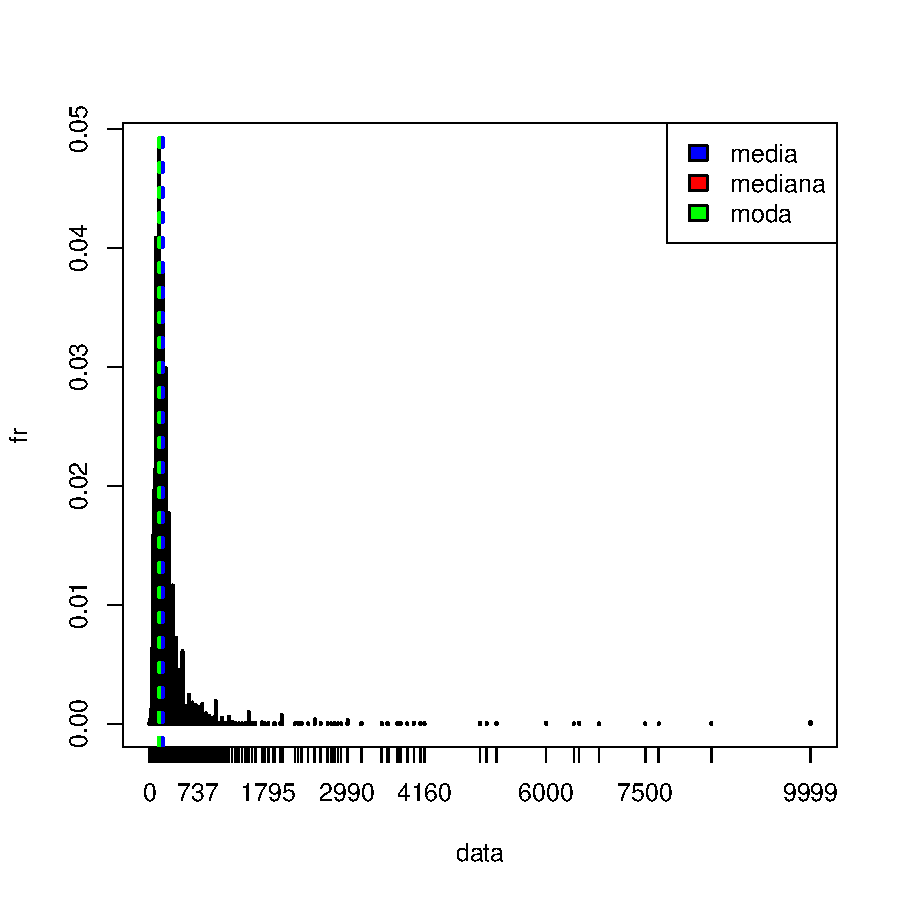
\includegraphics{entrega-029}
\end{center}
\begin{center}
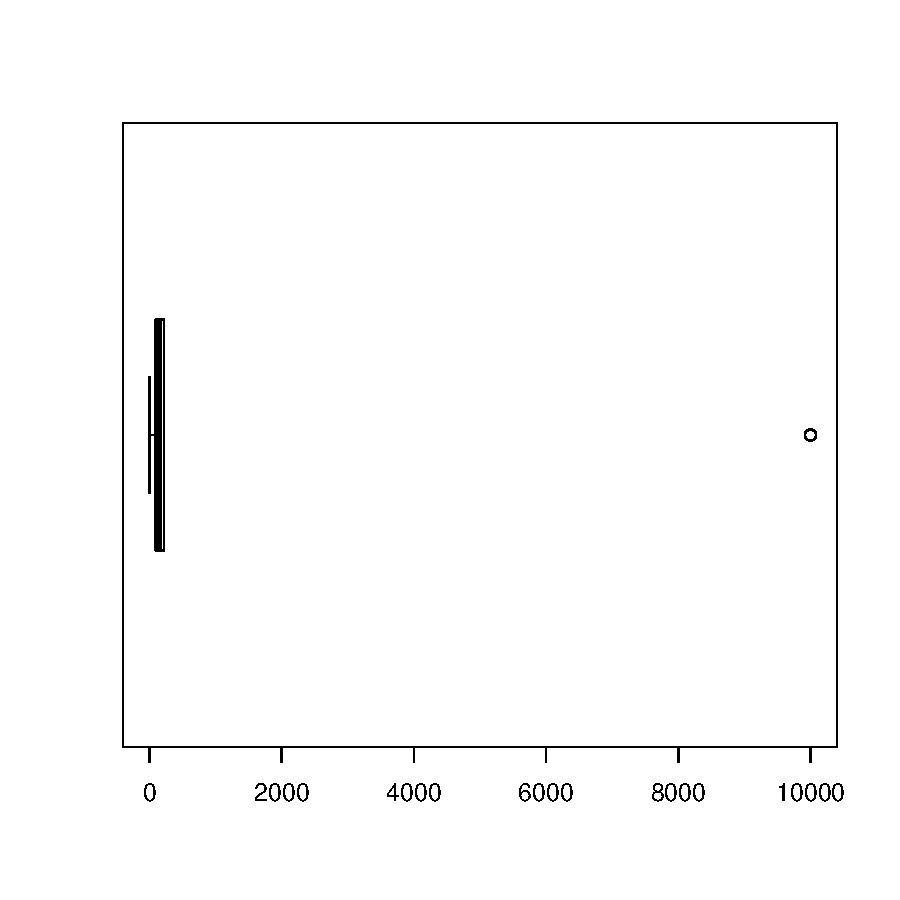
\includegraphics{entrega-030}
\end{center}

Datos para Bronx
\begin{center}
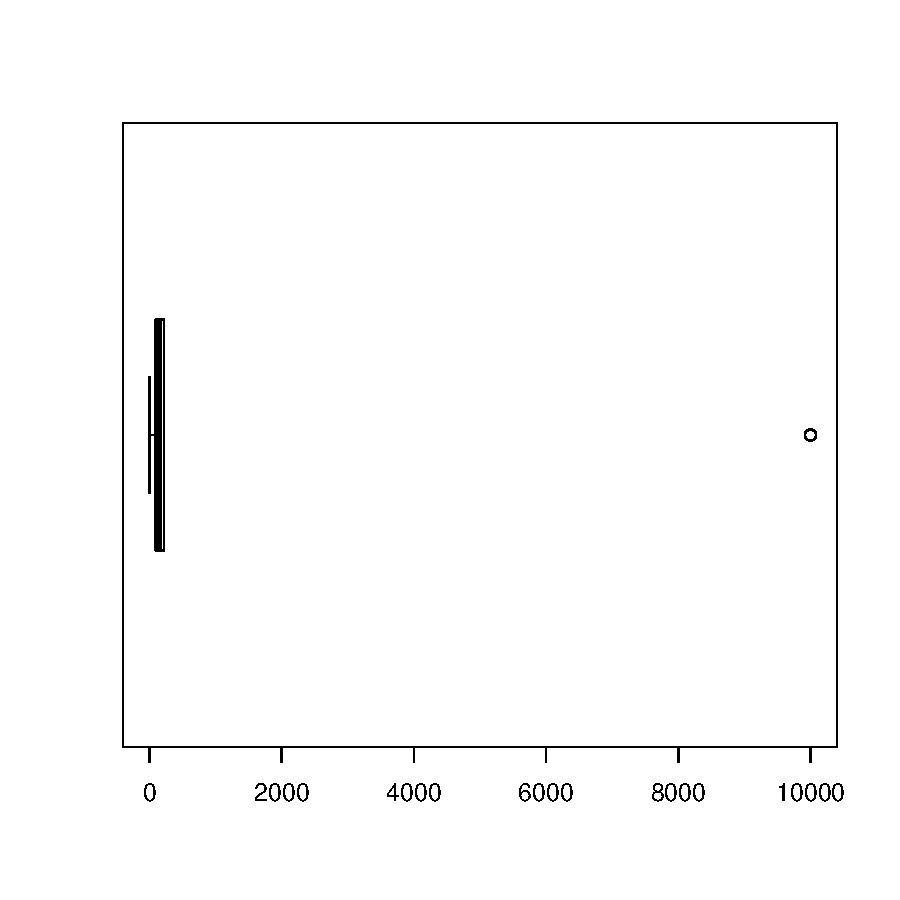
\includegraphics{entrega-031}
\end{center}
\begin{center}
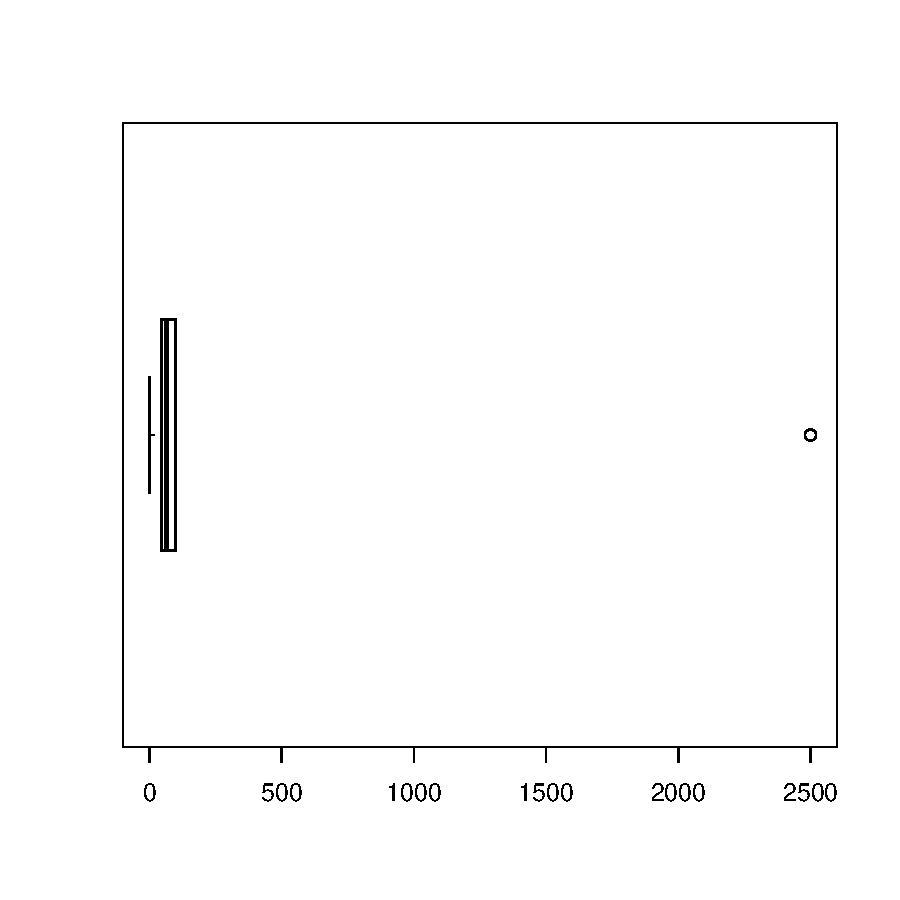
\includegraphics{entrega-032}
\end{center}

Datos para Brooklyn
\begin{center}
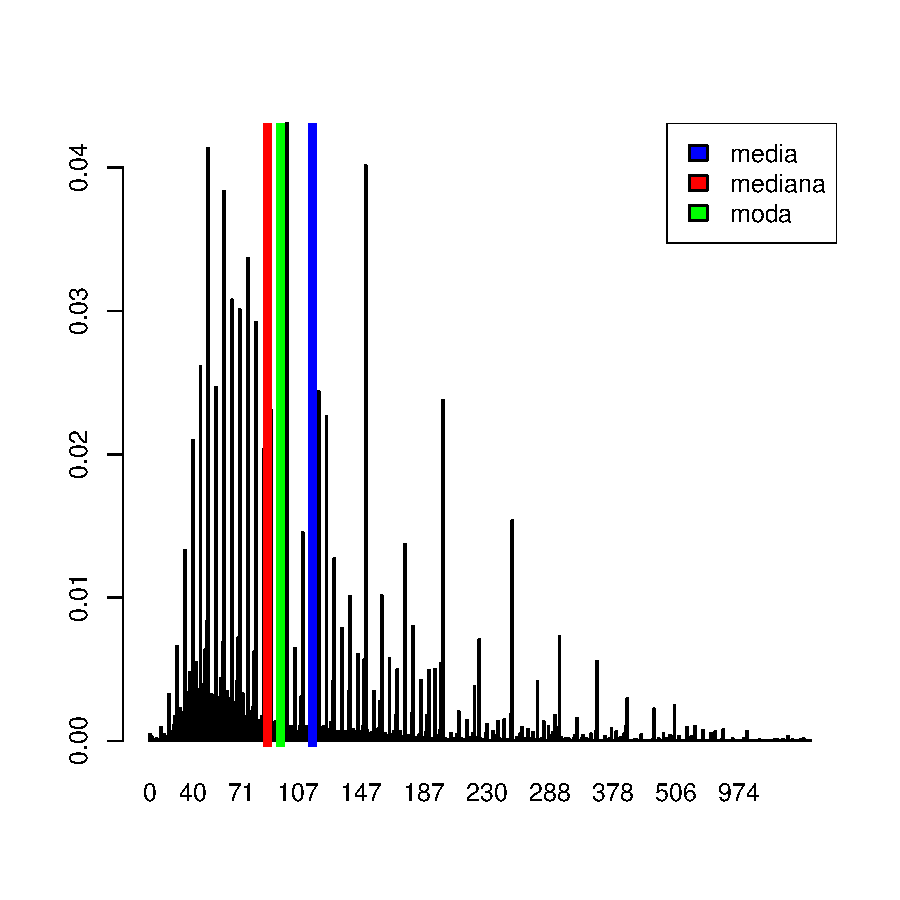
\includegraphics{entrega-033}
\end{center}
\begin{center}
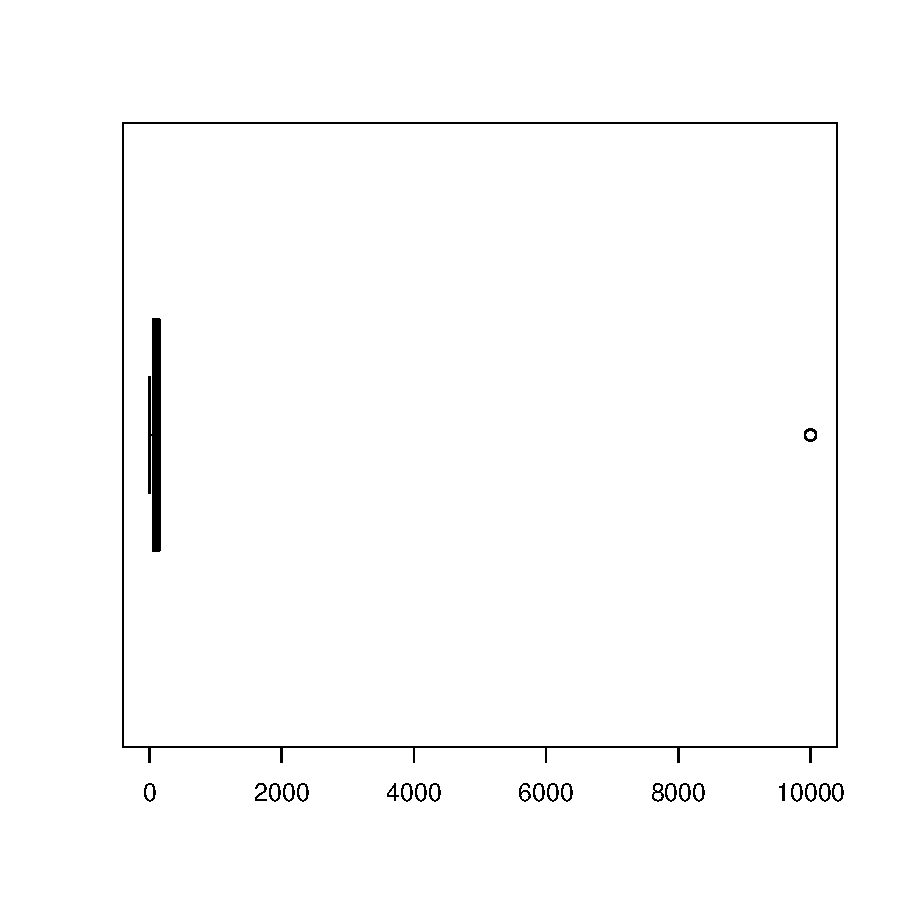
\includegraphics{entrega-034}
\end{center}

Datos para Queens
\begin{center}
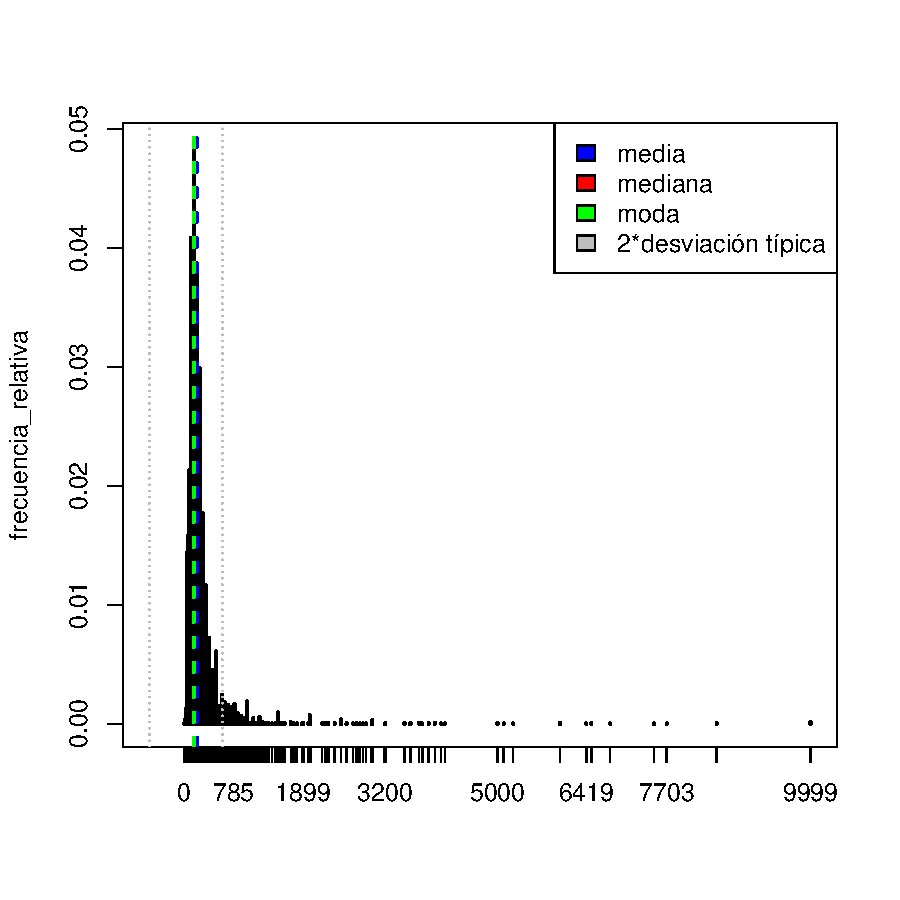
\includegraphics{entrega-035}
\end{center}
\begin{center}
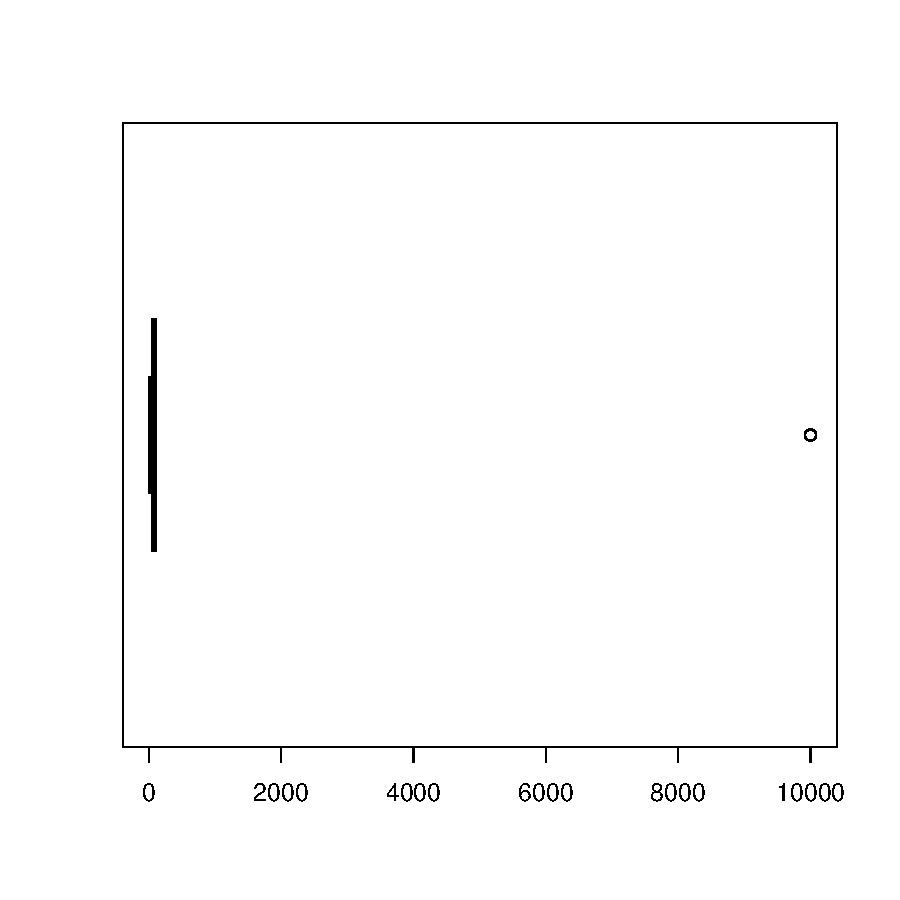
\includegraphics{entrega-036}
\end{center}

Datos para Staten Island
\begin{center}
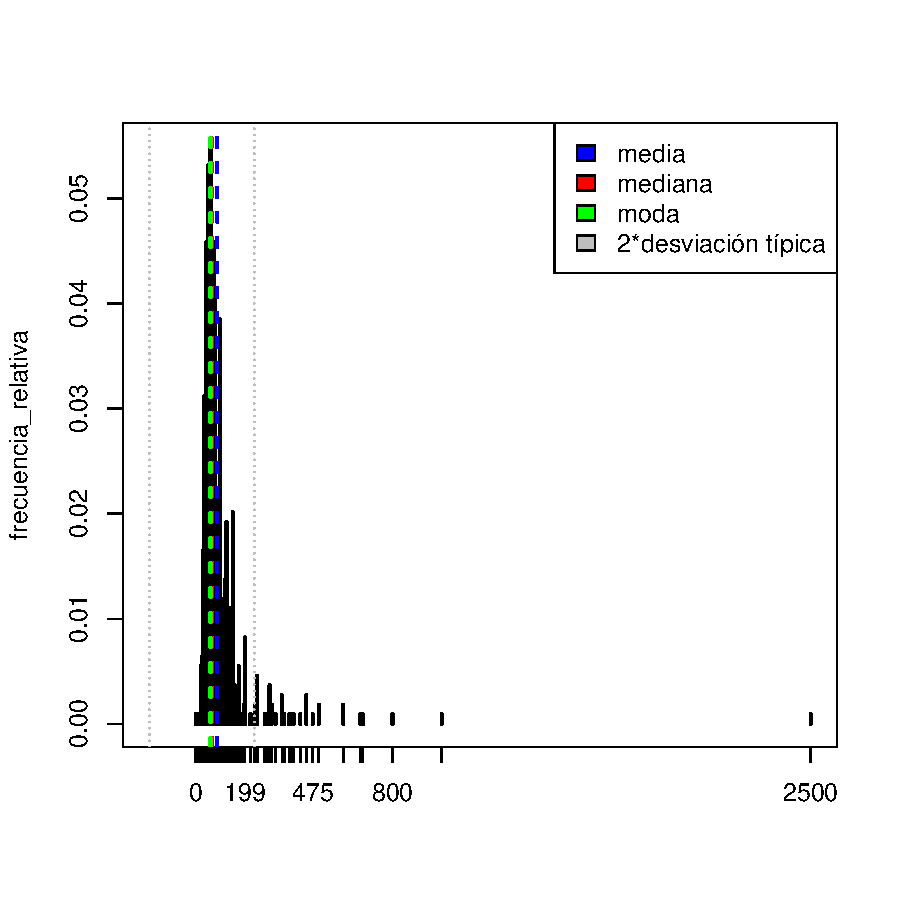
\includegraphics{entrega-037}
\end{center}
\begin{center}
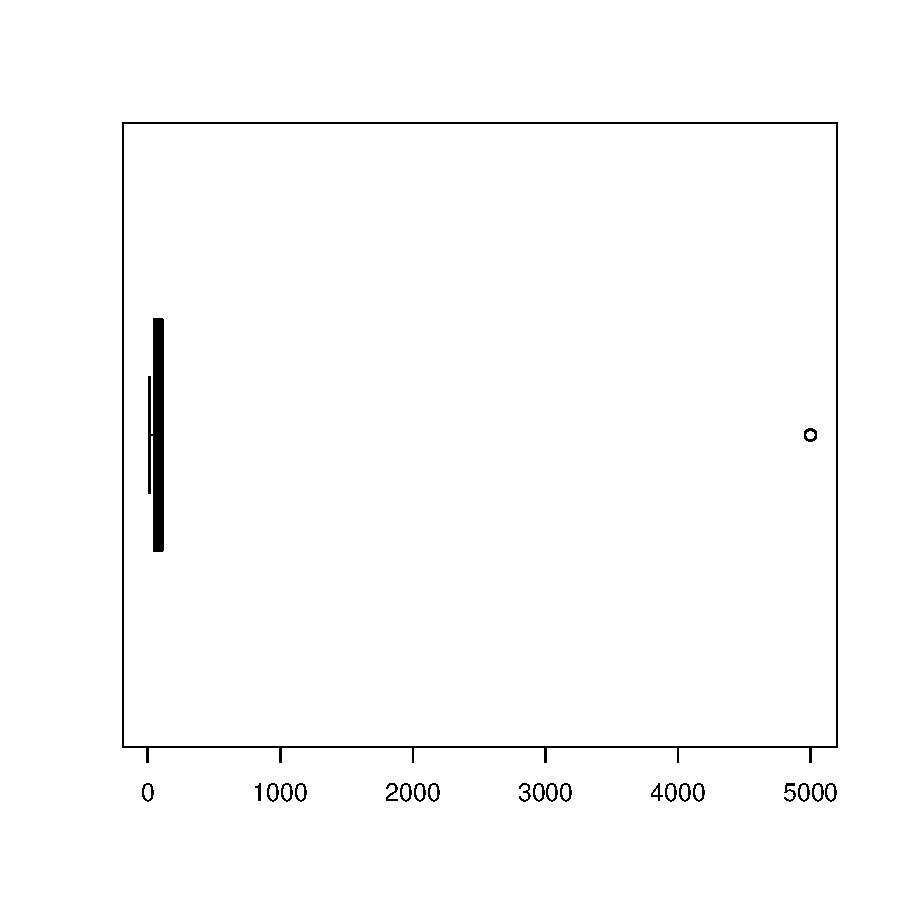
\includegraphics{entrega-038}
\end{center}
%-----------------------------------------------------------------------------------------------------------------------------------------------------------------------
\section{Guia en R para el análisis estadístico}
%-----------------------------------------------------------------------------------------------------------------------------------------------------------------------
\subsection{Frecuencias}
\begin{Schunk}
\begin{Sinput}
> Frecuencia_absoluta <- table(data)
> Frecuencia_absoluta_acumulada <- cumsum(frecuencia_absoluta)
> Frecuencia_relativa <- (function(data) table(data)/length(data))(data)
> Frecuencia_relativa_acumulada <- cumsum(frecuencia_relativa)
\end{Sinput}
\end{Schunk}
\subsection{Medidas representativas}
\begin{Schunk}
\begin{Sinput}
> Media <- mean(data)
> Desviacion_tipica <- sd(data)
> Varianza <- var(data)
\end{Sinput}
\end{Schunk}
\subsection{Medidas de ordenación}
\begin{Schunk}
\begin{Sinput}
> Mediana <- median(data)
> Cuartiles <- quantile(data, prob=c(0, .25, .5, .75, 1))
> Cuantil54 <- quantile(data, prob=(.54))
\end{Sinput}
\end{Schunk}

%-----------------------------------------------------------------------------------------------------------------------------------------------------------------------
\section{Funciones creadas}
%-----------------------------------------------------------------------------------------------------------------------------------------------------------------------
\subsection{Frecuencias}
\subsubsection{Frecuencia Absoluta}
\begin{Schunk}
\begin{Sinput}
> frecuenciaAbsoluta
\end{Sinput}
\begin{Soutput}
function(data){
  # creamos un vector donde solo estas los elementos sin repetir
  uniquedata<-unique(data)
  # ordenamos el vector para aparezco correcto 
  uniquedata<- sort(uniquedata)
  # creamos un vector vacio numerico
  newdata<- vector(mode="numeric", length=0)
  # recorremos el vector elementos no repetidos  
  for (value in uniquedata) {
    # calculamos la cantidad de veces que se repite un numero
    total<-length(data[data==value])
    # añadimos el total al vector con veces que se repitio
    newdata<-c(newdata, total)
  }
  # hacemos una matriz de tamaño 1xlongitud datos, añadimos los elementos la frecuencia
  matrix<-matrix(nrow=1,ncol=length(uniquedata), newdata, byrow=T)
  # en las filas ponemos el nombre que representa
  rownames(matrix)<-c("frecuencia")
  #en las columnas ponemos los datos
  colnames(matrix)<-c(uniquedata)
  #convertimos la matriz en una tabla
  matrix<-as.table(matrix)
}
<bytecode: 0x7fdf56451dc8>
\end{Soutput}
\end{Schunk}
\subsubsection{Frecuencia Absoluta Acumulada}
\begin{Schunk}
\begin{Sinput}
> frecuenciaAbsolutaAcumulada
\end{Sinput}
\begin{Soutput}
function(data){

    # calculamos la frecuencia
    frecuencia <-frecuenciaAbsoluta(data)
    # recuperamos el nombre de las columnas
    uniquedata<-colnames(frecuencia)
    # cogemos el vector de frecuencia
    onlydata<-frecuencia[1,]
    # creamos un vector vacio numerico
    newdata<- vector(mode="numeric", length=0)
    # recorremos desde la posicion 1 hasta lo maximo el vector
    for (value in 1:length(onlydata)) {
        # si el valor primero
        if(value==1){   
            # el acumulado es el mismo valor
            accumulated<-onlydata[value]
        # en otros casos
        }else{
            # el valor es anterior mas el valor suyo
            accumulated<-onlydata[value]+accumulated
        }
        # añadimos al vector el nuevo valor
        newdata<-c(newdata, accumulated)
    }
    # hacemos una matriz de tamaño 1xlongitud datos, añadimos los elementos la frecuencia
    matrix<-matrix(nrow=1,ncol=length(uniquedata), newdata, byrow=T)
    # en las filas ponemos el nombre que representa
    rownames(matrix)<-c("frecuencia acumulada")
    #en las columnas ponemos los datos
    colnames(matrix)<-c(uniquedata)
    #convertimos la matriz en una tabla
    matrix<-as.table(matrix)
}
\end{Soutput}
\end{Schunk}
\subsubsection{Frecuencia Relativa}
\begin{Schunk}
\begin{Sinput}
> frecuenciaRelativa
\end{Sinput}
\begin{Soutput}
function(data){
    #conseguimos frecuencia
    frecuencia <-frecuenciaAbsoluta(data)
    # recuperamos el nombre de las columnas
    uniquedata<-colnames(frecuencia)
    #cogemos solo el vector de frecuencia
    onlydata<-frecuencia[1,]
    #calculamos la suma total de frecuencia
    total<-sum(onlydata)
    #creo vector vacio numerico
    newdata<- vector(mode="numeric", length=0)
    #recorro todo el vector de datos
    for (value in 1:length(onlydata)) {
        # realizamos la division entre los datos y el total
        accumulated<-onlydata[value]/total
        # lo añado al nuevo array
        newdata<-c(newdata, accumulated)
    }
    # hacemos una matriz de tamaño 1xlongitud datos, añadimos los elementos la frecuencia
  matrix<-matrix(nrow=1,ncol=length(uniquedata), newdata, byrow=T)
  # en las filas ponemos el nombre que representa
  rownames(matrix)<-c("frecuencia relativa")
  #en las columnas ponemos los datos
  colnames(matrix)<-c(uniquedata)
  #convertimos la matriz en una tabla
  matrix<-as.table(matrix)
}
<bytecode: 0x7fdf55ac3998>
\end{Soutput}
\end{Schunk}
\subsubsection{Frecuencia Relativa Acumulada}
\begin{Schunk}
\begin{Sinput}
> frecuenciaRelativaAcumulada
\end{Sinput}
\begin{Soutput}
function(data){
    # calcumos la frecuencia acumulada
    frecuencia <-frecuenciaAcumulada(data)
    # recuperamos el nombre de las columnas
    uniquedata<-colnames(frecuencia)
    # cogemos el vector de frecuencia acumulada
    onlydata<-frecuencia[1,]
    # calculamos el total de datos 
    total<-onlydata[length(onlydata)]
    # creamos un vector vacio numerico
    newdata<- vector(mode="numeric", length=0)
    # recorremos desde la posicion 1 hasta lo maximo el vector
    for (value in 1:length(onlydata)) {
        #variable que calcula relativa entre la esa posicion entre total 
        relative<-onlydata[value]/total
        # añadimos al vector el nuevo valor
        newdata<-c(newdata, relative)
    }
    # hacemos una matriz de tamaño 1xlongitud datos, añadimos los elementos la frecuencia
  matrix<-matrix(nrow=1,ncol=length(uniquedata), newdata, byrow=T)
  # en las filas ponemos el nombre que representa
  rownames(matrix)<-c("frecuencia acumulada relativa")
  #en las columnas ponemos los datos
  colnames(matrix)<-c(uniquedata)
  #convertimos la matriz en una tabla
  matrix<-as.table(matrix)
}
\end{Soutput}
\end{Schunk}
\subsection{Medidas representativas}
Los siguentes valores pretenden ser representates de todos los datos que se estén analizando.
No tenemos garantís de que realmente lo sean así que para ellos necesitamos de erramientas que nos lo confiermen o desmientan.
\subsubsection{Media Aritmetica}
Suma ponderada por la cantidad de valores sumados.
Se podría haber utilizado la función sum que suma todos los valores de un vector en vez de haber iterado sobre ellos.
\begin{Schunk}
\begin{Sinput}
> mediaAritmetica
\end{Sinput}
\begin{Soutput}
function(data){
  acc <- 0
  for (value in data) {
    acc <- acc + value
  }
  acc / length(data)
}
<bytecode: 0x7fdf59920b98>
\end{Soutput}
\end{Schunk}
\subsubsection{Media Geométrica}
Raiz de orden igual a la cantidad de valores de la multiplicación de todos ellos.
El logaritmo de la media geométrica también puede expresarse como la media aritmética de los logaritmos de cada dato.
\begin{Schunk}
\begin{Sinput}
> mediaGeometrica
\end{Sinput}
\begin{Soutput}
function(data){
  prod(data)^(1/length(data))
}
\end{Soutput}
\end{Schunk}
\subsubsection{Media Armónica}
Inverso de la media de los inversos.
\begin{Schunk}
\begin{Sinput}
> mediaArmonica
\end{Sinput}
\begin{Soutput}
function(data){
  1/mediaAritmetica(1/data)
}
\end{Soutput}
\end{Schunk}
\subsubsection{Desviacion Típica}
Nos indica como de buena es la media aritmética. Cuanto menor sea la desviación mejor será la media.
Raiz cuadrada de la varianza.
\begin{Schunk}
\begin{Sinput}
> desviacionTipica
\end{Sinput}
\begin{Soutput}
function (data) {
  varianza(data)^(1/2)
}
<bytecode: 0x7fdf56781c10>
\end{Soutput}
\end{Schunk}
\subsubsection{Desviacion Media}
Nos indica como de buena es la media aritmética. Cuanto menor sea la desviación mejor será la media.
Se suele utilizar la desviacion típica en vez de la desviacion media.
Suma ponderada por la cantidad de valores del valor absoluto de los errores.
Se define error como la resta entre un valor y la media aritmética de todos ellos.
\begin{Schunk}
\begin{Sinput}
> desviacionMedia
\end{Sinput}
\begin{Soutput}
function (data){
  v_media <- media(data)
  acc = 0
  for (value in data){
    acc <- acc + abs(value - v_media)
  }
  acc/length(data)
}
\end{Soutput}
\end{Schunk}
\subsubsection{Varianza}
Nos indica como de buena es la media aritmética. Cuanto menor sea la varianza mejor será la media.
Suma ponderada por la cantidad de valores del cuadrado de los errores.
Se define error como la resta entre un valor y la media aritmética de todos ellos.
\begin{Schunk}
\begin{Sinput}
> varianza
\end{Sinput}
\begin{Soutput}
function(data){
  v_media <- mediaAritmetica(data)
  acc = 0
  for (value in data){
    acc <- acc + (value - v_media)^2
  }
  acc/length(data)
}
<bytecode: 0x7fdf54650560>
\end{Soutput}
\end{Schunk}
\subsubsection{Tchebychev}
Decir que la desviación típica es mejor cuanto menor sea no es demasiado precios.
El teorema de tchebychev nos proporciona una representación muy visual del significado de la media.
Se puede entender la media como un valor entorno al que se ubican los datos y la desviacion típica como una circunferencia con centro en la media y radio el valor de la desviación multiplicado por un factor K.
Tchebychev nos proporciona el porcentaje mínimo de valores que estarán dentro de cada valor de radio.
Esto nos ayuda a comparar la desviación obtenida con los datos que tratamos de una forma más significativa.
\begin{Schunk}
\begin{Sinput}
> tchebychev
\end{Sinput}
\begin{Soutput}
function(data, limit=10){
  desviacion_tipica = desviacionTipica(data)
  for (k in 2:limit){
    data_percentage <- (1-(1/k^2))*100
    radious = desviacion_tipica*k
    message(paste("En un radio de",radious,"se encuentran el",data_percentage,"de los datos, k=",k))
  }
}
\end{Soutput}
\end{Schunk}
\subsection{Medidas de ordenación}
\subsubsection{Mediana}
La mediana la hemos calculado ordenando los datos en orden ascendente 
y obteniendo el punto que se encuentra en la mitad de ese vector 
o la media entre los 2 puntos que se encuentran en este lugar.
\begin{Schunk}
\begin{Sinput}
> mediana
\end{Sinput}
\begin{Soutput}
function(data){
  x = sort(data)
  size = length(x)
  if (size  %% 2 == 0){
    (x[size / 2] + x[(size / 2) +1]) / 2.0
  }
  else {
     x[size / 2]
  }
}
<bytecode: 0x7fdf55c62168>
\end{Soutput}
\end{Schunk}
\subsubsection{Cuartiles}
Los cuartiles los hemos calculado ordenando los datos en orden ascendente 
y obteniendo los 3 puntos que dividen el vector en 4 partes iguales, es decir, 
el cuartil 25, el 50 y el 75.
\begin{Schunk}
\begin{Sinput}
> cuartiles
\end{Sinput}
\begin{Soutput}
function(data){
    x = sort(data)
    size = length(x)
    if (size  %% 2 == 0){
        c(
            x[1],
            (x[size / 4] + x[(size / 4) +1]) / 2.0 ,
            (x[size / 2] + x[(size / 2) +1]) / 2.0 ,
            (x[size *0.75] + x[size * 0.75 + 1]) / 2.0,
            x[size]
        )

    }
    else {
        c(
            x[1],
            x[size / 4],
            x[size / 2],
            (x[size *0.75] + x[size * 0.75 + 1]) / 2.0,
            x[size]
        )
  }

}
<bytecode: 0x7fdf54c2bbc0>
\end{Soutput}
\end{Schunk}
\subsubsection{Cuantil54}
El cuantil 54 los hemos calculado ordenando los datos en orden ascendente 
y obteniendo el punto en el que detrás de él se encuentran el 54% de los datos. 
\begin{Schunk}
\begin{Sinput}
> cuantil54
\end{Sinput}
\begin{Soutput}
function(x){
  size = length(x)
  x[ceiling(size*0.54)]
}
\end{Soutput}
\end{Schunk}

\end{document}
